\documentclass[a4paper]{article}
\pdfoutput=1
\usepackage[utf8]{inputenc}
\usepackage{jheppub}
\usepackage{overpic}
\usepackage{subcaption}
\usepackage{fancybox}
\usepackage{float}
\usepackage{amsfonts}
\usepackage{amsmath}
\usepackage{amsbsy}
\usepackage{graphicx}
\usepackage{amssymb}
\usepackage{amsthm}
\usepackage{bm}
\usepackage{comment}
\usepackage{epsfig}
\usepackage{latexsym}
\usepackage{pdflscape}
\usepackage{color}
\usepackage{stmaryrd}
\usepackage{tikz}
\usetikzlibrary{arrows.meta,decorations.markings}

\tikzset{
  mid arrow/.style={
    postaction={
      decorate,
      decoration={
        markings,
        mark=at position 0.5 with {\arrow{Stealth[length=6pt,width=6pt]}}
      }
    }
  }
}

\usepackage{cancel}
\usepackage{xcolor}
\usepackage{braket}
\usepackage{empheq}
\usepackage{graphicx} % Allows including images
\usepackage{tikz-3dplot}
% réglage de la vue 3D : élévation=20°, azimut=110°
\tdplotsetmaincoords{20}{110}
\usetikzlibrary{decorations.pathreplacing,calc}
\usetikzlibrary{decorations.pathmorphing}

\definecolor{blue5}{rgb}{0, 0, 0.66666}
\definecolor{red4}{rgb}{0.8, 0, 0}
\definecolor{navyblue}{rgb}{0, 0.2745, 0.67843}
\definecolor{cornflowerblue}{rgb}{0.388235, 0.6941176, 0.898039}
\definecolor{forestgreen}{rgb}{0.13, 0.55, 0.13}
\usetikzlibrary{decorations.text,decorations.pathmorphing}

%Removes Header------------------------------------
\makeatletter
\def\@fpheader{\relax}
\makeatother



\usepackage{orcidlink}

%\DeclareMathOperator{\tr}{tr}
\DeclareMathOperator{\pf}{pf}
\DeclareMathOperator{\Ai}{Ai}
\DeclareMathOperator{\vol}{vol}
\DeclareMathOperator{\sgn}{sgn}
\DeclareMathOperator{\sn}{sn}
\DeclareMathOperator{\cn}{cn}
\DeclareMathOperator{\dn}{dn}
\DeclareMathOperator{\cd}{cd}
\DeclareMathOperator{\Det}{Det}
\DeclareMathOperator{\sech}{sech}
% \DeclareMathOperator{\tr}{tr}

\newcommand{\beq}{\begin{eqnarray}}
\newcommand{\eeq}{\end{eqnarray}}
\newcommand{\bea}{\begin{eqnarray}}
\newcommand{\eea}{\end{eqnarray}}
\newcommand{\be}{\begin{equation}}
\newcommand{\ee}{\end{equation}}
\newcommand{\bq}{\begin{equation}}
\newcommand{\eq}{\end{equation}}
\newcommand{\unit}{1\!\!1}
\newcommand{\half}{\frac{1}{2}}
\newcommand{\nn}{\nonumber}
\newcommand{\no}{\nonumber}
\def\tb{\tilde{\beta}}
\newcommand{\mpl}{M_{\rm Pl}}
\def\k{\kappa}

\newcommand{\bto}{\bar{\tau}^{\textbf{I}}}
\newcommand{\btt}{\bar{\tau}^{\textbf{II}}}




%%% Other definitions


\def\sp{\;\;\;,\;\;\;}
\def\l{\lambda}
%\def\z{\zeta}
\def\lab{\label}
\def\f{H}
\def\La{\Lambda}
\def\z{\zeta}
\def\t{\tau}
\def\e{\epsilon}
\def\o{\omega}
\def\le{\left}
\def\ri{\right}
\def\y{\psi}
\def\half{\frac12}
\def\q{\theta}
\def\cO{{\cal O}}
\def\m{\mu}
\def\n{\nu}
\def\td{\tilde}
\def\d{\delta}
\def\6{\partial}
\def\de{\partial}
\def\del{\nabla}
\def\ls{\ell_s}
\def\a{\alpha}
\def\b{\beta}
\def\lab{\label}
\def\parl{\parallel}
\def\tom{\tilde{\o}}
\def\dA{\dot{A}}
\def\dh{\dot{h}}
\def\df{\dot{f}}
\def\dX{\dot{X}}
\def\bo{\bar{\o}}
\def\r{x}
\def\bo{b_0}
\def\br{\bar{r}}
\def\dx{\delta X^\parl}
\def\dxy{\delta X^2}
\def\dxz{\delta X^3}
\def\ol{\overline}
\def\GM#1{\textit{[GM: #1]}}
\def\g{\gamma}
\def\s{\sigma}
\def\tr{{\rm Tr}}
\def\eps{\epsilon}
\def\fb{f}
\def\rd{\rm d}
\newcommand{\bom}[1]{\fboxsep2mm\fbox{
           $ \displaystyle{ #1} $}}
           
           \newcommand{\rar}{\rightarrow}
\newcommand{\bb}{\mathbb}
\newcommand{\mc}{\mathcal}
\newcommand{\im}{\mathrm{Im}}
\newcommand{\re}{\mathrm{Re}}
\newcommand{\mi}{\sqrt{|\mathcal{I}_4|}}


\def\lab{\label}
\def\le{\left}
\def\ri{\right}
\def\6{\partial}
\def\eps{\epsilon}


% Color definitions
\newcommand{\red}[1]{{\color{red} #1 \color{black}}}
\newcommand{\blue}[1]{{\color{blue} #1 \color{black}}}
\newcommand{\green}[1]{{\color{green} #1 \color{black}}}
\newcommand{\yellow}[1]{{\color{yellow} #1 \color{black}}}
\newcommand{\purple}[1]{{\color{purple} #1 \color{black}}}


% Comment Abbreviations
\newcommand{\IT}[1]{{\red{IG: #1}}} %Ioannis
\newcommand{\PB}[1]{{\blue{PB: #1}}} % Panos
\newcommand{\OP}[1]{{\green{OP: #1}}} % Olga
\newcommand{\PG}[1]{{\purple{PG: #1}}} % Paul

\title{Entanglement entropy in c=1 non critical string theory}

\author[a]{Panos Betzios\orcidlink{0000-0002-5350-9404},}
\author[b]{Paul Ghiringhelli,}
\author[b]{Olga Papadoulaki\orcidlink{0000-0001-5302-2930}}
\affiliation[a]{\href{https://www.ugent.be/we/physics-astronomy/en}{Department of Physics and Astronomy},
Ghent University, \\ Krijgslaan, 281-S9, 9000 Gent, Belgium}
\affiliation[b]{\href{https://www.cpht.polytechnique.fr/?q=en}{CPHT, CNRS, École polytechnique, Institut Polytechnique de Paris},  91120 Palaiseau, France}

\emailAdd{panos.betzios@ugent.be}
\emailAdd{paul.ghiringhelli@polytechnique.edu}
\emailAdd{olga.papadoulaki@polytechnique.edu}





\abstract{...}

\keywords{...}


\begin{document}
\maketitle
\flushbottom


%%%%%%%%%%%%%%%%%%%%%%%%%%%%%%%%%%%%%%%%%%%%%%%%%%%%%%%%%%
\cite{boutivas2025numericalcalculationentanglemententropy}\cite{Boutivas_2023}\cite{Boutivas_2024}\cite{ginsparg1993lectures2dgravity2d}\cite{Bombelli:1986rw}\cite{Bombelli:1986rw}
\cite{headrick2019lecturesentanglemententropyfield}
\section{Continuum theory}

\subsection{From the sigma model to the gauge fixed action.}
At the level of the worldsheet, $c=1$ non critical strings is described by a scalar coupled to two-dimensional Euclidean gravity, with a cosmological constant and a topological Einstein term on a smooth, compact two dimensional manifold $\mathcal{M}_h$ with genus $h$ and metric $g$.
\begin{equation}\label{eq:worldsheetaction}
\mathcal{S}_{\sigma}^{(h,g,\Phi_0)}=\frac{1}{4\pi}\int_{\mathcal{M}_h} d^2 x \sqrt{g}\left(g^{\mu \nu}\partial_\mu X \partial_\nu X +\Phi_0\mathcal{R}+4 \pi \mu\right)\,.
\end{equation}
$\Phi_0$ is a constant and is connected to the constant part of the linear dilaton background. The Gauss-Bonnet theorem states that $\frac{1}{4\pi}\int d^2x \sqrt{g}\mathcal{R}$ is a topological number known as the Euler characteristic $\chi_h=2-2h$. The partition function is defined through the path-integral over all possible metrics on $\mathcal{M}_{h}$ modulo Diffeomorphism and the boson $X$
\begin{equation}
  \mathcal{Z} = \sum _{h\geq0} (g_0)^{-\chi_h} \int \frac{[Dg^{(h)}_{\mu \nu}]}{\text{Vol}(\text{Diffeo})} [DX]e^{-\mathcal{S}_{\sigma}^{(h,g)}}\,,
\end{equation}
where we introduced the notation $g_0 = e^{\Phi_0}$. We can gauge fix the metric to the fiducial metric $g_{\mu \nu}=e^{2b\phi}\hat{g}_{\mu \nu}^{(\tau)}$. The price to pay is the introduction of b, c ghost fields. The measure is not invariant under the previous map. Also, the cosmological constant term yields a non trivial $\phi$ dependence (because of the cosmological constant term, even classically Weyl symmetry is broken). Combined together, they yield the Liouville action
\begin{equation}
  \mathcal{S}^{(\hat{g}_h)}_{L}=\frac{1}{4\pi}\int d^2x \sqrt{\hat{g}_h}\left(\hat{g}^{\mu \nu}_h \partial_\mu \phi \partial_\nu \phi +Q \hat{\mathcal{R}}\phi+4\pi\mu e^{2b\phi}\right)\,.
\end{equation}
In the case of $c=1$ matter boson 
\begin{equation}
    c_L = 1+6Q^2 = 1+ 6(b+b^{-1})^2 = 26-c = 25\,.
\end{equation}
but we keep everything general at this stage. The remaining integral to perform is an integral over the conformal mode $\phi$ known as the Liouville field and an integral over the moduli space parametrized by $\tau$. Hence, the partition function finally reads
\begin{equation}\label{eq:finalgaugefixing}
  \begin{aligned}
    \mathcal{Z} = \sum _{h\geq0} (g_0)^{-\chi_h} \int d\tau \int [D\phi][DX][Db][Dc]e^{-(\mathcal{S}_{\sigma}+\mathcal{S}_{b,c}+\mathcal{S}_{L})}\,,
  \end{aligned}
\end{equation}
where $V_{h}$ is the volume of the moduli space of $M_h$. 

Let's focus on the Liouville sector for a moment. We can exploit that $\phi$ is integrated over to extract the $\mu$ dependence of the Liouville partition function~\cite{martinec2004matrixmodels2dstring}. In fact, assuming the measure is invariant under $\phi \rightarrow \phi -\frac{\log(\mu)}{2b}$, one obtains
\begin{equation}\label{eq:KPZ}
  \mathcal{Z}^{(h)}_L(\mu) = \mu^{\frac{Q\chi_h}{2b}}\mathcal{Z}^{(h)}_L(\mu = 1)\,.
\end{equation}
This is the genus expansion of the partition function. In the case of interest $c=1,\,Q=2,\,b=1$, we simply have an expansion in $\mu$. As we will review later the cosmological constant is realted to the string coupling at the position of the Liouville wall $g_{\rm{s}}(\phi = \phi_\star) \sim \mu^{-1}$. As for the rest of the paper, we will now focus on the case $c_L=1,\,c=1$. The spectrum of normalizable states of $c_L = 25$ Liouville theory reads (the integral indicates a direct sum)
\begin{equation}
    \mathcal{H} = \underset{\oplus}{}\int_0^{+\infty} dp_L \mathcal{V}_{p_L} \otimes \bar{\mathcal{V}}_{p_L}\,,
\end{equation}
where $\mathcal{V}_{p_L}$ correspond to the highest weight representations of the Virasoro algebra and $p_L$ is the Liouville momentum related to the conformal dimension by
\begin{equation}
    \Delta_L = \frac{Q^2}{4}+p_L^2 = 1 +p_L^2\,.
\end{equation}
As is it well known the identity operator $p_L=i\frac{Q}{2}$.

On the matter side, The Hilbert space consists in the closed-string fock-space obtained by acting with creation/annhilitation operators on the closed-string vacuum. A particular important set of operators in our latter discussion is what we define as \textit{pseudo-tachyon} vertex operator defined by
\begin{equation}\label{eq:pseudo-tachyon}
    \mathcal{O}_{k}(X) = :e^{i k X}:\,.
\end{equation}
They are associate with primary states with conformal dimension $\Delta=\frac{k^2}{4}$. We refer to them as \textit{pseudo-tachyon} as the momentum $k$ is not assigned to a specific value but may be related to the Liouville momentum due to the Virasoro constraint.

\subsection{Liouville action and Target space interpretation} The different terms appearing in the Liouville+matter action have a meaning in terms of Target space fields. Let's recall the general form of the generalized non linear sigma model in presence of a dilaton $\Phi(Y)$, a Tachyon condensate $T(Y)$ and non trivial metric $G_{\mu \nu}(Y)$.
\begin{equation}
  \mathcal{S} = \frac{1}{4\pi}\int d^2x \sqrt{\hat{g}}\left(T(Y)+\hat{\mathcal{R}}\Phi(Y)+g^{ab}G_{\mu \nu}\partial_a Y^\mu \partial_b Y^\nu\right)\,.
\end{equation}
We see by comparison to the Liouville + matter action that $Y = (X,\phi)$ and
\begin{equation}\label{eq:background}
  T = 4\pi \mu e^{2 \phi}\sp G_{\mu \nu} = \delta_{\mu \nu}\sp  \Phi= \Phi_0+2\phi\,. 
\end{equation}
Remark that we effectively started with a sigma model with one boson and landed on a theory which has now two bosons $X,\phi$. We say that from the non-decoupling of the conformal mode, a new dimension has emerged. This describes a inhomogeneous 2D space $(\phi,X)$. Such inhomogeneity emerges in the $\phi$ direction due to the Liouville potential. The string coupling depends on the value of the dilaton and thus on the position in the $\phi$ direction as the dilaton and the Liouville conformal mode are related by~\eqref{eq:background}. An observer sitting on the Liouville wall defined by the condition
\begin{equation}\label{eq:relationLiouvillewallcosmologicalconstant}
  \mu e^{2_\star} = 1 \Rightarrow \Phi_\star = \Phi_0 + 2\phi_\star = \Phi_0 -\log(\mu)\,.
\end{equation}
observes the scattering of states with the string coupling $g_\star = e^{\Phi_\star}$. The amplitude of the process should be perturbatively described by a genus expansion in the string coupling at the position of the Liouville wall. This is exactly what the KPZ scaling relation gives (see~\eqref{eq:finalgaugefixing},~\eqref{eq:KPZ}).

This is important to note that the background~\eqref{eq:background} is solution of the one-loop vanishing of the $\beta$ functions only for $\mu=0$. For $\mu\neq0$ the Liouville interaction should be interpreted as a tachyon-wall background rather than as a naive linear-dilaton solution of the free beta-function equations.
\PG{We need to add more stuff on Target space vs string field theory. This is important to cite also~\cite{Balasubramanian_2018} since I got the idea of looking at the string field reading this paper.}

\subsection{BRST constraint/Wheeler De Witt equation and physical states}
In principle, the Hilbert space of the final gravitational theory Liouville/matter/ghosts corresponds exactly to a BRST cohomology of the total state space $\mathcal{H}_{\rm tot}=\mathcal{H}_{\rm Liouville}\otimes \mathcal{H}_{\rm matter}\otimes\mathcal{H}_{\rm ghost}$, precisely
\begin{equation}
    \mathcal{H}_{\rm phys} = H^{\bullet}\left(Q_{\rm BRST}, \mathcal{H}_{\rm tot}\right)\,.
\end{equation}
It is well known that, in non-critical string theory, the physical Hilbert space contains an infinite tower of discrete states, the Lian--Zuckerman states, whose ghost number is non-zero\PG{Cite modern discussions here}. In what follows, we discard these states and restrict attention to the projection of the physical Hilbert space onto the zero-ghost-number sector. Since $\mathcal{H}_{\rm tot}$ is diagonal, it is enough to consider the holomorphic sector. In this sector, the BRST constraint reduces to
\begin{equation}
    \left(L_0^{(\phi)} + L_0^{(X)} - 1\right)\ket{\Psi}=0\,.
\end{equation}
This condition applied on the tensor product of primary states imposes the marginality condition $\Delta_L +\Delta_X =1$.
\paragraph{Minisuperspace truncation}
Consider now the theory on the cylinder. Minisuperspace consists in imposing that the fields do not depend on the circular direction 
\begin{equation}
    \phi(\tau,\sigma)=\phi_0(\tau)\, \qquad X(\tau,\sigma)=X(\tau)\,.
\end{equation}
At the level of the Hilbert space, this means on the matter side that we discuss only the level $0$ space spanned by operators of the form~\eqref{eq:pseudo-tachyon} and on the Liouville side we consider projecting each Verma module onto its highest weight state. Consider now the case of a tensor product state of primaries
\begin{equation}\label{eq:tensorprimaries}
    \ket{\Psi} = \ket{\mathcal{O}_{k}}\otimes \ket{\Psi_{p_L}}\,.
\end{equation}
The marginality condition imposes $\Delta_X+\Delta_L =1 \Rightarrow k = 2ip_L$. Hence the truncation of the physical Hilbert space to minisuperspace leads to (focusing on the left moving part only)
\begin{equation}\label{eq:minihilbert}
\begin{aligned}
    \mathcal{H}_{\rm mini/ phys}
    &=L^2\left(\mathbb{R}_{x}\times \mathbb{R}^{+}_{\ell}, d\mu = dx\frac{d\ell}{\ell}\right)\\
    &= \underset{\oplus}{}{\int_0^{+\infty} }\rm{d}p_L \,\ket{\mathcal{O}_{2ip_L}}\otimes \ket{\Psi_{p_L}}\,.\\
\end{aligned}
\end{equation}
Let's describe in further details the Liouville states for $c_L=1$. The genus zero minisuperspace Lagrangian on the cylinder is
\begin{equation}
\begin{aligned}
     L_{\rm zero-mode} = \frac{1}{2}\left((\partial_\tau \phi_0)^2 + 4\pi \mu e^{2b \phi_0}\right)\\
     L_{\rm zero-mode} = \frac{1}{2}\left((\partial_\tau \phi_0)^2 + 4\pi \mu e^{2 \phi_0}\right)
\end{aligned}
\end{equation}
It has been argued that at the quantum level the Hamiltonian has to be normal ordered and that the normal ordering procedure may affect the form of the hamiltonian by introducing terms like~\cite{teschner2000remarksliouvilletheoryboundary} $\mu e^{2\phi/b}$ in order for the $b\to1/b$ duality to be recovered at the quantum level. The authors would like to emphasize that for $c=1,\,c_L=25$, we have $b=1$ and thus $c=1$ non critical strings is a fixed point of the duality relation.
Applying canonical quantization on the cylinder the Schrodinger equation is\begin{equation}\label{eq:Schrodinger}
 \left[-\frac{1}{2}\frac{\partial^2}{\partial{\phi_0}^2}+2\pi \mu e^{2b\phi_0}\right]\Psi_{p_L}(\phi_0)=2 p_L^2 \Psi_{p_L}(\phi_0)\,.
\end{equation}
Introducing the loop parameter $\ell = e^{\phi_0}$, this becomes a modified Bessel equation
\begin{equation}\label{eq:Wheeler-De-Witt-spacelike}
  \ell^2\frac{\partial^2}{\partial{\ell}^2}\Psi_{p_L}(\ell)+\ell\frac{\partial}{\partial{\ell}}\Psi_{p_L}(\ell)-\left(\frac{4\pi\mu}{b^2}\ell^2-\frac{4p_L^2}{b^2}\right)\Psi_{p_L}(\ell)=0\,.
\end{equation}
States that decay in the strong coupling region $\phi_0\to \infty$ correspond to Bessel-K functions. So,
\begin{equation}
  \Psi^{(p)}_L(\ell) \propto K_{\frac{2ip_L}{b}}\left(\frac{2\sqrt{\pi\mu}}{b}\ell\right)\,.
\end{equation}
At this stage, this is common to define $E = 2p_L$ so that in the weak coupling region for $c=1 \Rightarrow b=1$, we have a superposition of incoming and outgoing plane waves $e^{\pm i\phi E}$. As it should be, this is even in $p$ (or $E$) so that $\Delta_L$ is indeed the correct physical parameter. By definition,
\begin{equation}
  K_{\nu}(z)=\frac{I_{\nu}(z)-I_{-\nu}(z)}{\sin(\pi \nu)}\,,
\end{equation}
and we have the asymptotics $I_{\nu}(z)\underset{z\to 0}{\sim} \left(\frac{z}{2}\right)^\nu$. We further define the reflection coefficient such that asymptotically in the weak coupling region
\begin{equation}
  \Psi_{p_L}(\ell) \underset{\ell \to 0}{\propto} e^{2ip_L\phi_0}+ R(p_L)e^{-2ip_L\phi_0}\,.
\end{equation}
Due to the expression of $K_\nu$ and the asymptotic expansion of $I_\nu$, we find
\begin{equation}
  R(p_L)=-\sin\left(\pi\frac{2ip_L}{b}\right)\times \left(\frac{\pi \mu}{b^2}\right)^{2ip_L/b}\,.
\end{equation}
In what follow, we will focus on the case $c=1\Rightarrow b=1$.
\PG{Leg factors and blabla this is important to say something at this point. the third quantized theory would be the same but with a renormalized vacuum. I think it is related to these leg factors.}

\paragraph{Genus 0 minisuperspace string field action}
In the limit of low energy, the BRST operator exacty reduces to the minisuperspace Wheeler-De-Witt operator. The low energy limit restricts attention to region of the $\phi$ space before the Liouville wall. Topology changing processes and non local effects are thus expected to become important in the high energy regime. \PG{In the weak coupling region $\phi\to\infty$, the BRST constraint reduces to the Wheeler-De-Witt operator and locality is recovered.}
\begin{equation}\label{eq:simpleentanglemententropy}
  \mathcal{S}_{\rm third} =  \frac{1}{2} \int \rm{d}\phi \rm{d}X \left[\left(\partial_\phi \Psi\right)^2+ \left(\partial_X \Psi\right)^2+4\pi \mu e^{2b\phi}\Psi^2\right]\,.
\end{equation}
We shall view this as a massive field theory whose mass is expressed in terms of the string coupling $m^2 = 2\sqrt{\pi \mu}e^{b\phi} \sim g_s(\phi)$ which depends on the position in the $\phi$ space. In particular, in the strict weak coupling region, it describes a massless scalar field theory in 1+1 dimension. We therefore immediatly obtain that the entanglement entropy of the vacuum of a cut $A=[\phi_1,\phi_2]$ in the weak coupling region is given by Cardy-Calabrese universal~\cite{Pasquale_Calabrese_2004} law
\begin{equation}
  S^{\rm c=1}_A = \frac{1}{3}\log\left(\frac{\phi_2-\phi_1}{\epsilon_{\rm UV}}\right)+c\,,
\end{equation}
where $c$ is a non universal constant and $\epsilon_{\rm UV}$ is a UV-cutoff. Since the $\phi$-position sets the energy scale of the problem, the Liouville potential can naturally be expressed as a RG flow equation for the mass
\begin{equation}
  \frac{d m(\phi)}{d\phi} = b\, m(\phi)\,.
\end{equation}
\paragraph{Numerical method for computing the EE}
\PG{If we consider a finite size systen $[\phi_1,\phi_2]$, it actually becomes important whether we impose Neumann or Dirichlet boundary conditions at the endpoints! What shall we choose ?}
\paragraph{A first exercise to benchmark our numerical analysis: Entanglement entropy of a massive scalar field in 1+1d.}
We consider a massive scalar field $\phi$ in 1+1d. The hamiltonian of such system is
\begin{equation}
\begin{aligned}
     H &= \frac{1}{2}\int \rm{d}x \,\left[\pi_\phi^2 + (\partial_x \phi)^2 + m^2 \phi^2\right]\,.
\end{aligned}
\end{equation}

The entanglement entropy of a quantum field theory is not well defined as the entanglement entropy between adjoining spacetime regions is UV divergent~\cite{Witten_2018}. To circumvulate such problem, we consider a discretize/lattice version of the previous model. Let $a$ be the lattice spacing in the x-direction. Note that
\begin{equation}
  \phi(x+a) - \phi(x) = a \partial_x \phi + \mathcal{O}(a^2)\,.
\end{equation}
The idealized situation that we should mimic is the infinite line. Numerically, the field is represented by a finite dimensional vector whose size matches the size of the lattice. One way to retrieve the infinite line results is to consider the theory on the circle (or in other word, we impose periodic boundary conditions) and consider large radius with respect to the entanglement cut. An other possibility is to consider open boundary conditions, that is we do not impose any boundary conditions. We can thus associate to the afforementionned QFT the following lattice model.
\begin{equation}
  H = \frac{1}{2a^2} \sum \pi_n^2 + \left(\phi_{n+1}-\phi_n\right)^2 + m^2 a^2 \phi_n^2\,.
\end{equation}
A method first described by Srednicky~\cite{Srednicki_1993} and Bombelli and al.~\cite{Bombelli:1986rw} can be systematically applied to such lattice system. For a recent review, see for instance~\cite{Casini_2009}\cite{bellucci2026entanglemententropymassivescalar}\cite{Boutivas_2023}\cite{Boutivas_2024}. In these preliminary works, they show that the entanglement entropy of the vacuum state for a massless scalar field in flat space is proportional to the area. The method consists in writting the Hamiltonian as
\begin{equation}
  \tilde{H} = \frac{1}{2}\sum_m \pi_n^2 + \frac{1}{2}\sum_{i\,j}\phi_i K_{ij}\phi_j\,,
\end{equation}
with
\begin{equation}
\begin{aligned}
  K^{\text{periodic}}_{ij}&= \delta_{ij}\left(\tilde{m}^2 + 2\right)-\left(\delta_{i j+1}+ \delta_{i j-1}\right)\,,\\
  K^{\text{open}}_{ij}&= \delta_{ij}\left(\tilde{m}^2 + 2\right)-\left(\delta_{i j+1}+ \delta_{i j-1}\right)- \delta_{i n_i} \delta_{j n_j} - \delta_{i n_f} \delta_{j n_f}\,.
\end{aligned}
\end{equation}
To simplify notations, we droped the lattice prefactor in front of the hamiltonian and we define the lattice mass $\tilde{m}^2=m^2 a^2$. The matrix $K$ is a positive definite symmetric matrix (provided $m^2>0$). The crucial difference is that $K^{\text{periodic}}$ is not exactly tridiagonal but has non zero elements in the corners compared to $K^{\text{open}}$ which is tridiagonal but has $1+ m^2$ in both endpoints instead of $2+m^2$. The method consists in taking its square-root on a finite but large size interval (large compared to the entanglement subregion in order to prevent side effects) compared to the subregion of the entanglement entropy. Then, the entropy is easily computed from the eigenvalues of the $C$ matrix on the spatial subregion $A$ where $C$ is defined as
\begin{equation}
  C_{|A} = \sqrt{\braket{\phi \phi}_{|A} \braket{\pi \pi}_{|A}}  = \frac{1}{2}\sqrt{\left(K^{-1/2}\right)_{|A} \left(K^{1/2}\right)_{|A}}\,.
\end{equation}
For numerical stability, it is easier to determine the eigenvalues of $C^2_{|A}$ and then to diagonalize. Denoting $\nu_k$ the eigenvalues of $C_{|A}$, the entanglement entropy of the vacuum state reads
\begin{equation}
  S = \sum_k \left(\nu_k+\frac{1}{2}\right)\log\left(\nu_k +\frac{1}{2}\right) - \left(\nu_k-\frac{1}{2}\right)\log\left(\nu_k -\frac{1}{2}\right)
\end{equation}
Finite size effects were studied and the entanglement entropy of a cut for the ground state for a system of size $L$ with periodic boundary conditions is reads~\cite{Calabrese_2009}~\cite{Pasquale_Calabrese_2004}
\begin{equation}\label{eq:entropysizeeffects}
\begin{aligned}
  S_{A,\text{periodic}}&=\frac{c}{3}\log\left(\frac{L}{\pi a}\sin\left(\frac{\pi \ell}{L}\right)\right)+c\,,\\
  S_{A,\text{open}}&=\frac{c}{6}\log\left(\frac{L}{\pi a}\sin\left(\frac{\pi \ell}{L}\right)\right)+2g+c\,.
\end{aligned}
\end{equation}
where $c$ is a non universal contribution and $g$ is the boundary entropy term found by Affleck and Ludwig~\cite{Affleck:1991tk}. These formula are actually very efficient when one wants to extract the central charge of a critical system in 1+1 dimension. By fitting the numerical data with~\eqref{eq:entropysizeeffects}, we can extract the central charge. The following plots show the results of such a procedure for both boundary conditions.

\begin{figure}[!h]
  \centering
  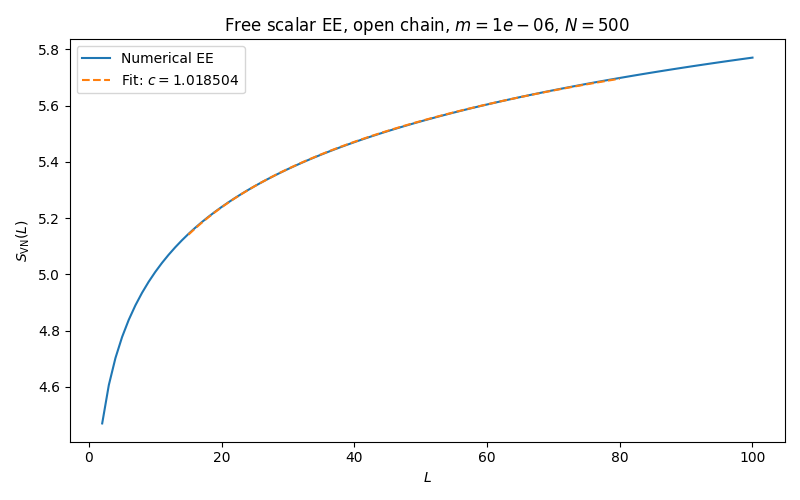
\includegraphics[width=0.6\linewidth]{open_freescalar.png}
  \caption{Fit of the entanglement entropy curve as a function of the size of the cut imposing open boundary conditions}
  \label{fig:open_freescalar}
\end{figure}


\begin{figure}[!h]
  \centering
  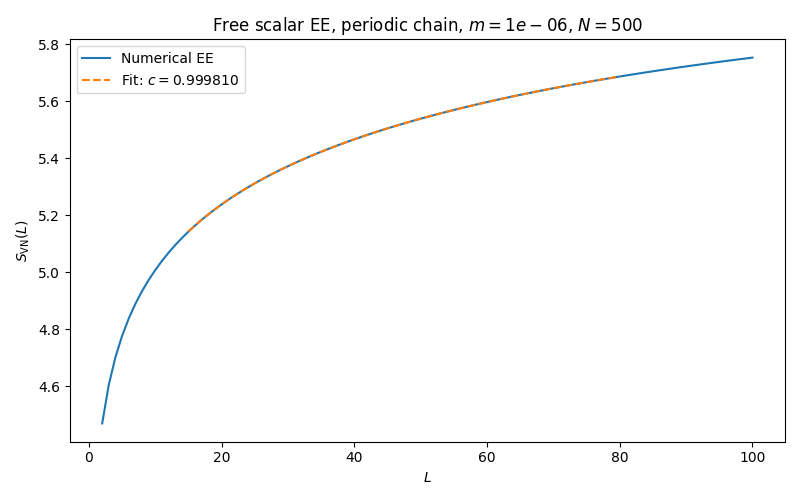
\includegraphics[width=0.6\linewidth]{periodic_freescalar.png}
  \caption{Fit of the entanglement entropy curve as a function of the size of the cut imposing periodic boundary conditions}
  \label{fig:periodic_freescalar}
\end{figure}


\paragraph{EE in minisuperspace genus $0$ approximation.}
A discretized version of the action~\eqref{eq:simpleentanglemententropy} is simply given by ($\phi_n=n a$ is the lattice coordinate)
\begin{equation}
  H = \frac{1}{2a^2}\sum_n \pi_n^2 +(2+m_n^2 a^2)\Psi_n^2 -(\Psi_n\Psi_{n+1}+\Psi_n\Psi_{n-1})+\text{endpoint contribution}\,,
\end{equation}
The theory is not translation invariant along the spatial coordinate $\phi$, it thus does not make any sense to impose periodic boundary conditions.
with $m_n^2 = 4\pi \mu e^{2 n a b}$. For the $c=1$, after dropping the lattice prefactor, this yields
\begin{equation}
  \tilde{H} = \frac{1}{2}\sum_m \pi_n^2 + \frac{1}{2}\sum_{i\,j}\phi_i K^{L}_{ij}\phi_j\,,
\end{equation}
with
\begin{equation}
  K^{L}_{ij}= \delta_{ij}\left(4\pi \tilde{\mu} e^{2 a i} + 2\right)-\left(\delta_{i j+1}+ \delta_{i j-1}\right)\,.
\end{equation}
We introduced the lattice bare cosmological constant $\tilde{\mu} = \mu a^2$. Two things are important to notice. First, this is no more translation invariant. Second, the mass aspect depends on the lattice spacing and we can't get rid of it.
\paragraph{A note regarding Zamolodchikov c-theorem and subadditivity}
Zamolodchikov c-theorem states that for any local unitary QFT in 1+1d translationnaly and rotationnaly invariant the $c$ function is increasing~\cite{Zamolodchikov:1986gt}\cite{Casini_2007}. We emphasize here that translation in $\phi$ space is explicitly broken by the presence of this exponential factor and thus we do not expect the c-theorem to apply for the function
\begin{equation}
  c(\phi_L,\phi_R) = 3(\phi_R-\phi_L)\frac{\rm{d} S}{\rm{d}(\phi_R -\phi_L)}\,.
\end{equation}
In particular, as is it clear from the numerics, such a function would be negative at some point ruining the interpretation of the c-function as capturing the number of degrees of freedom.

In Lorentz invariant field theory, the growth of the c-function is tied to the strong subadditivity property. Let us inspect the consequence of the SSA in a non translation invariant QFT. Let three spacetime regions $A,B,C$. Whatever state you start with, the SSA reads
\begin{equation}\label{eq:SSA}
  S(ABC)-S(BC)-\left(S(AB)-S(B)\right) \leq 0\,.
\end{equation}
Let $A=[\phi_L-\delta \phi_L, \phi_R - \delta \phi_R],\,B =[\phi_L, \phi_R],\, C=[\phi_L+\delta \phi_L, \phi_R + \delta \phi_R]$.
We have
\begin{equation}
\begin{aligned}
  &S(ABC)-S(BC)-\left(S(AB)-S(B)\right) \\
  &= S[\phi_L-\delta \phi_L, \phi_R + \delta \phi_R] - S[\phi_L, \phi_R + \delta \phi_R] -\left(S[\phi_L- \delta \phi_L, \phi_R]- S[\phi_L, \phi_R]\right)\\
  &=-\delta \phi_L \frac{\partial S}{\partial \delta \phi_L}[\phi_L,\phi_R + \delta \phi_R] + \delta \phi_L \frac{\partial S}{\partial \delta \phi_L}[\phi_l, \phi_R]\\
  &= -\delta \phi_L \delta \phi_R \frac{\partial ^2 S}{\partial \delta \phi_L \partial \delta \phi_R}\,.
\end{aligned}
\end{equation} 
In particular,~\eqref{eq:SSA} leads to the positivity of the Hessian. For the discretized lattice field theory, we can check the SSA criteria by taking $\delta \phi_L = a = \delta \phi_R$. \PG{I checked that by printing a boolean: I first construct a grid of entropy values in terms of two discretized variables $\phi_L, \phi_R$ and then I construct a matrix corresponding to the LHS of~\eqref{eq:SSA}. Then, I check non-positivity of the entries of the matrix. I can make a 3D plot if you wish...}

\paragraph{The relation between the minisuperspace action and the Klein gordon theory in 1+1 dimension}\label{par:relationminiKG}
Consider $t=-iX$ as the time variable and $\phi$ as the space variable. The minisuperspace Lorentzian action is obtained from the Euclidean action~\eqref{eq:simpleentanglemententropy} and reads
\begin{equation}
  \mathcal{S}_{\rm{L,\,third}} = \frac{1}{2} \int \rm{d}\phi \rm{d}X \left[\left(\partial_t \Psi\right)^2-\left(\partial_\phi \Psi\right)^2 -4\pi \mu e^{2b\phi}\Psi^2\right]\,.
\end{equation}
Perform now the substitution $T = e^{\phi}\sinh(t),\,\bar{X} = e^{\phi}\cosh(t)$. We obtain the following action
\begin{equation}
\begin{aligned}
    S_{\rm{KG}} = \frac{1}{2}\int \rm{d}T \rm{d}\bar{X} \left[\left(\partial_T \Psi\right)^2 -\left(\partial_{\bar{X}} \Psi\right)^2 - 4\pi \mu \Psi^2\right]\,.
\end{aligned}
\end{equation}
We land on a massive Klein-Gordon theory in 1+1 dimension with mass $m^2 = 4\pi \mu = \frac{4\pi}{g_{s}(\phi = \phi_\star)}$. As a check of such correspondence, we can observe that the Klein-Gordon equation expressed in terms of $(\phi,\,t)$ reproduces the minisuperspace Wheeler-De-Witt equation~\eqref{eq:Wheeler-De-Witt-spacelike} providing we identified the frequency of the Klein-Gordon mode $\omega$ with $2p_L$ as was suggested by the marginality condition see~\eqref{eq:minihilbert}. It has been argued that the problems of the Wheeler-De-Witt equation are very similar to the Klein-Gordon equation. Here such correspondence is made explicit.\PG{Include citations here}.

The vacuum of the original minisuperspace field theory~\eqref{eq:simpleentanglemententropy} is defined to be the unique state annhilated by the Hamiltonian which is the conserved charged associated with invariance under time-translation in $t$. Lines of constant $\phi$ are mapped to trajectories for which $X^2-T^2=\text{const}$ which describes hyperboloids. The Killing vector $\xi$ is the boost Killing vector in $T,\bar{X}$ variable as we also have $\xi = T\partial_{\bar{X}} + T\partial_{\bar{X}}$. To summurize, the pure state vacuum of the original theory is obtained by tracing out the left-wedge degrees of freedom of the pure state Rindler vaccum of the Klein-Gordon theory in 1+1d. 
\begin{equation}
  \rho_{\rm{KG}} = \underset{\beta \to +\infty}{\lim}\frac{e^{-\beta H_{R}}}{\text{Tr}\left[e^{-\beta H_{R}}\right]} = \ket{0_R}_{\rm{R}} {}_{\rm{R}}\bra{0_R}\,.
\end{equation}
$\ket{0_R}_{\rm{R}}$ is the right Rindler vacuum and $H_{R}$ is the modular boost Hamiltonian restricted to the right Rindler wedge
\begin{equation}
  H_R = \int_{0}^{+\infty} X T_{00}(T=0,X) \rm{d}X = \int_{0}^{+\infty} \rm{d}\omega \,\omega b_{\omega}^{\dagger, R} b_{\omega}^{R}\,. 
\end{equation}
For a recent review on the the Rindler vacuum and the Unruh effect, see~\cite{Crispino_2008}~\cite{Higuchi_2017}~\cite{Birrell:1982ix}.
\subsection{The Hilbert space structure of the truncated minisuperspace third quantized field theory.}
\PG{We should say something at some point regarding LZ states and the fact that here we only focus on the physical states with ghost excitation = 0}
The minisuperspace truncation consists in keeping zero-mode excitations both on the Liouville side and on the matter side. Concerning the matter side, it means that we exactly allow states mapped to pseudo-Tachyon closed-strings vertex operators $\mathcal{V}_k = e^{i k X}$. We refer to them as pseudo-Tachyon vertex opetors as they formally take the same expression as the tachyon vertex operator but here $k$ is not entirely fixed. Regarding the Liouville sector, this projects each each Verma module onto its highest weight state i.e primary state. The physical Hilbert space described by the minisuperspace quantum mechanics thus consists of a tensor products of such states submitted to the WdW constraint which is the marginality condition $\Delta_X + \Delta_L =1$
\begin{equation}
  \mathcal{H}_{\text{mini}} = \int_{0}^{+\infty} dp_L \ket{\Psi^{X}_{2i p_L}} \otimes \ket{\Psi^{L}_{p_L}}\,.
\end{equation}
\paragraph{Dependence on the choice of state.}
The Von Neumann entropy we numerically compute is associated to the vacuum and pure state $\rho = \ket{0}\bra{0}$ uniquely defined to be the state annihilated by the hamiltonian with flow parameter $t=iX$ of the third quantized action. Let us detail such procedure. We introduce an orthonormal basis of the WdW using the Kontorovich-Lebelev transform
\begin{equation}
  \begin{aligned}
    \psi_E(\ell) &= \frac{1}{\pi}\sqrt{\pi \sinh(\pi E)}K_{iE}(2\sqrt{\pi \mu}\ell)\,,\\
    \int_{0}^{+\infty} &\frac{\rm{d}\ell}{\ell}\psi_E(\ell)\psi_{E'}(\ell) = \delta(E-E')\,.
  \end{aligned}
\end{equation}
We then decompose the third quantized fields in terms of the elements of the basis
\begin{equation}
  \Psi(\phi=\log(\ell),t=iX)=\int_0^{+\infty}\frac{dE}{\sqrt{2E}} \,\psi_E(\ell) \left(a_{E}e^{-i\omega(E) t }+a^{\dagger}_{E}e^{i\omega(E) t }\right)\,.
\end{equation}
The dispersion relation is given by the WdW and yields $\omega(E)^2=E^2$. Even though the action is not translation invariant in $\phi$, it remains translation invariant in $X$. Thus, the Hamiltonian
\begin{equation}
\begin{aligned}
    H &= \int_0^{+\infty} \frac{\rm{d}\ell}{\ell} \left[\frac{1}{2}\left(\partial_t \Psi\right)^2 + \frac{\ell^2}{2}\left(\partial_\ell \Psi\right)^2 + 2\pi \mu e^{2 \phi} \Psi^2\right]\\
    &=\int_0^{+\infty} \frac{\rm{d}\ell}{\ell} \left[\frac{1}{2}\left(\partial_t \Psi\right)^2 + \frac{1}{2}\Psi\left(-\mathcal{H}_\ell \right)\Psi\right]\,.
\end{aligned}
\end{equation}
is a conserved quantity. We then rewrite the Hamiltonian in terms of the oscillator modes and we normal order to obtain
\begin{equation}
  H = \int_0^{\infty} dE E a^{\dagger}_{E} a_{E}\,.
\end{equation}
The vacuum $\ket{0}$ is uniquely defined (up to a phase) to be the state annihilated by the hamiltonian equivalently by all the oscillators. Only in this case does the point function reads
\begin{equation}
  \bra{0}\Psi(\ell,t)\Psi(\ell',t)\ket{0} =\int_0^{+\infty} \frac{dE}{2E} \Psi_E(\ell) \Psi_E'(\ell') = \frac{1}{2}\left(-\mathcal{H}_\ell\right)^{-1/2} (\ell,\ell')\,.
\end{equation}
If one describes the system in angular variable $w=e^{\phi +i X}$, define $T = \frac{w+\bar{w}}{2}, Y = \frac{w - \bar{w}}{2}$ so that to rewrite the action in the form of a KG action and subsequently define the new vacuum by asking the Haniltonian with flow parameter T to annihilated such a state, you compute EE of a different state.

\appendix
\section{Replica trick}
The replica trick is a method used to compute the von-Neumann entropy of a quantum system defined by the density matrix $\rho$. This was initially developped in~\cite{Callan_1994}\cite{Holzhey_1994} and later generalized in~\cite{Calabrese_2009}. The idea is to compute the Renyi-entropy of order $n$ defined as
\begin{equation}
  S_A^{(n)} = \frac{1}{1-n}\log\left(\text{Tr}\left[\rho_A^n\right]\right)\,.
\end{equation}
and then take the limit $n\to1$ to obtain the Von-Neumann entropy. It takes its name from the fact that the computation of $\text{Tr}\left[\rho_A^n\right]$ can be interpreted as a path-integral over an $n$-sheeted Riemann surface $\mathcal{R}_n$ with branch cuts along the entanglement region $A$. Consider the original theory defined on the complex plane. For a single interval $A=[u,v]$, the partition function on the $n$-sheeted Riemann surface is expressed in terms of a two-point function of twist fields $\mathcal{T}_{n},\mathcal{\tilde{T}}_{n}$ on the upper-half plane $\mathbb{H}$
\begin{equation}
  \text{Tr}\rho_A^n = \frac{Z_n(A)}{Z^n} \propto \braket{\mathcal{T}_{n}(u,0)\mathcal{\tilde{T}}_{n}(v,0)}_{\mathbb{H}}\,.
\end{equation}
The recipe consists in noting that the twists operators are primaries with conformal dimensions $\Delta_{n} = \frac{c}{12}\left(n-\frac{1}{n}\right)$. 

\subsection{Replica trick for the minisuperspace third quantized field theory}
Consider the theory defined by the action~\eqref{eq:simpleentanglemententropy}. In the weak coupling region, this theory describes a CFT in 1+1 dimension with central charge $c=1$. We thus expect to obtain the universal Cardy-Calabrese law
\begin{equation}
  S_{A} = \frac{1}{3}\log\left(\frac{\phi_1-\phi_2}{\epsilon_{UV}}\right)\,,
\end{equation}
if $\phi$ is far way from the Liouville wall. 

But we can gain more information through the map described in~\ref{par:relationminiKG}. We may further assume that $\mu \ll 1$ which is essentially true at genus $0$. Then, Both theories can be considered as a CFT in 1+1 dimension. While this statement may be seen to be trivial, it is actually a way to compute corrections to the previous formula. Defining, $z = \phi + i X$ and $w = e^{z}$, we obtain 
\begin{equation}
  \braket{\mathcal{T}_{n}(\phi_1,0)\mathcal{\tilde{T}}_{n}(\phi_2,0)}_{\text{mini}} = |w'(\phi_1)w'(\phi_2)|^{\Delta_n} \braket{\mathcal{T}_{n}(w(\phi_1),0)\mathcal{\tilde{T}}_{n}(w(\phi_2),0)}_{\text{KG}}\,.
\end{equation}
Hence
\begin{equation}
  \braket{\mathcal{T}_{n}(w(\phi_1),0)\mathcal{\tilde{T}}_{n}(w(\phi_2),0)}_{\text{KG}} = \frac{(\phi_1-\phi_2)^{2\Delta_n}}{\left(e^{\phi_1}e^{\phi_2}\right)^{\Delta_n}}\,.
\end{equation}
With $g_{s}= e^{2\phi}$, we obtain
\begin{equation}
  S_{A} = \frac{1}{3}\log\left(\frac{\phi_1-\phi_2}{(g_s(\phi_1)g_{s}(\phi_2))^{1/4}}\right)\,.
\end{equation}

\bibliographystyle{JHEP}
\bibliography{biblio}

\end{document}